\def \imgpath {"./figures/sphero"}
In this chapter, measurements of \KOs, \LA, and \AL are reported as a function of transverse spherocity \SOPT. It is defined as
\begin{align}
\SOPT = \frac{\pi^2}{4} \min_{\hat{n}} \left(\frac{\sum_i
      |\hat{p_{\textrm{T},i}} \times \hat{n}|}{N_{\textrm{trks}}}  \right) \quad ,
\end{align}
where $\hat{p_{\textrm{T},i}}$ represents the unit vector of transverse momentum of a particle $i$, $N_{\textrm{trks}}$ the number of charged particles entering the sum, and $\hat{n}$ is the event-dependent unit vector which minimises the sum. The sum runs over all charged particles in the event within $|\eta|<0.8$ and with $\pt > 0.15$~\gevc \ .
\section{Understanding transverse spherocity}

TBA: Illustrating isotropic and jetty event.

TBA: Motivation for studying \SOPT

TBA: Motivation for unweighted spherocity

\begin{figure}%
\subfloat[][]{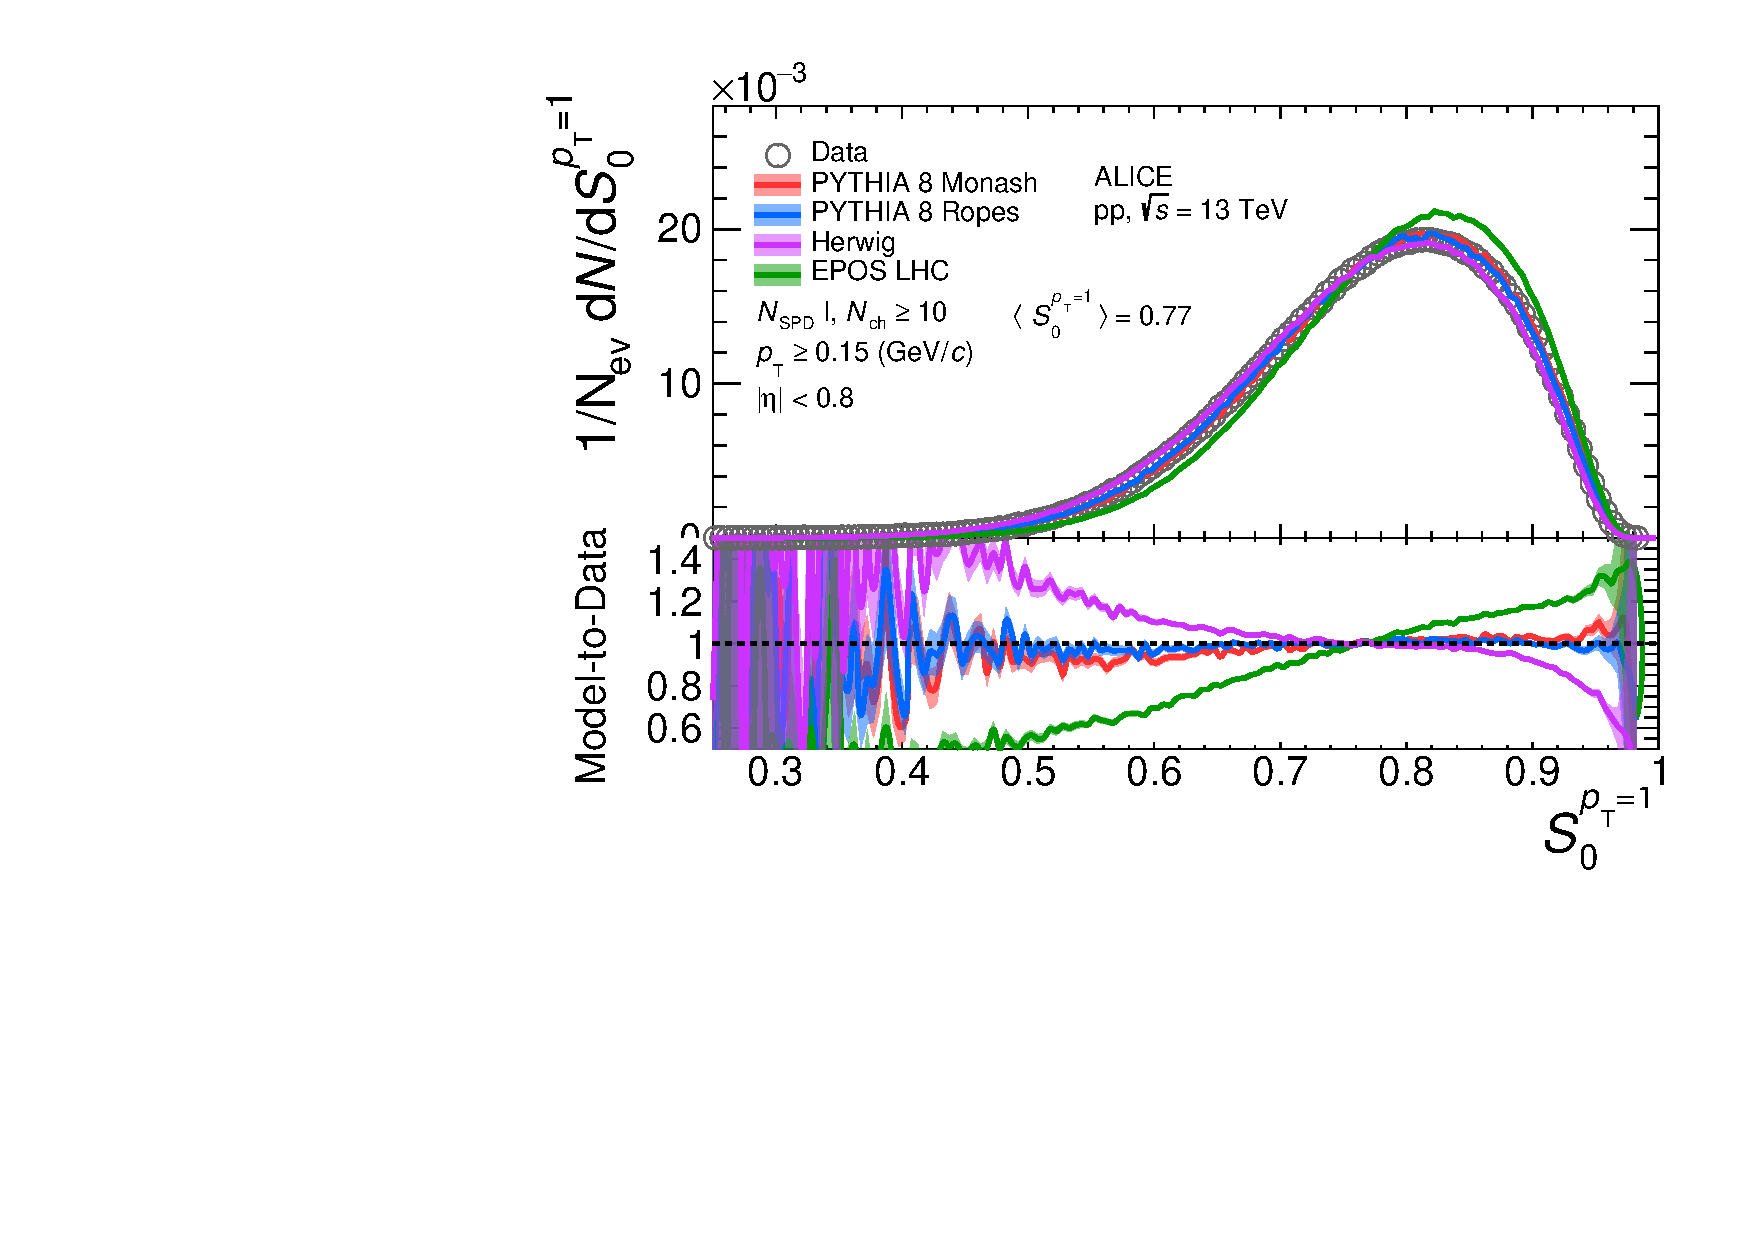
\includegraphics[width=.60\textwidth]{\imgpath/SO_Unfolded_CL1_Perc_1.pdf}}\\
\subfloat[][]{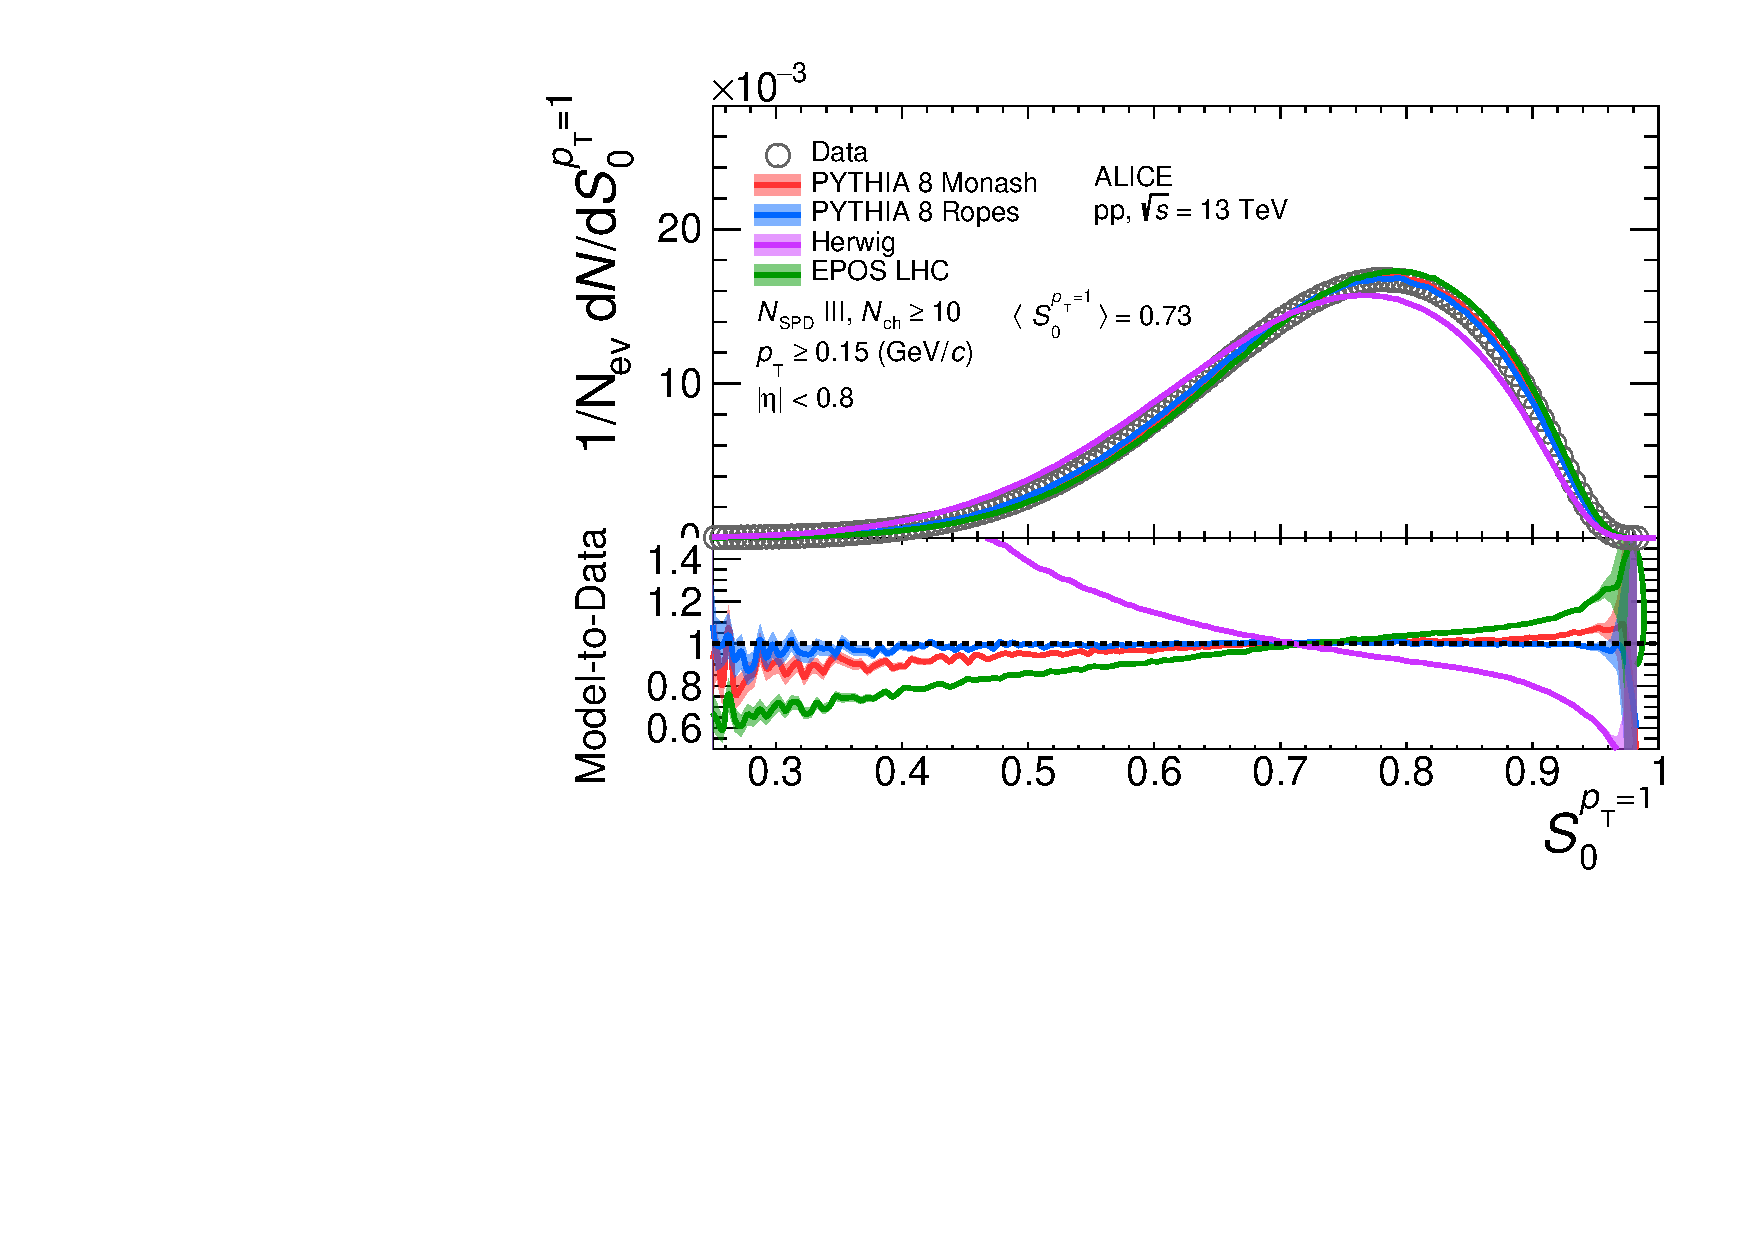
\includegraphics[width=.60\textwidth]{\imgpath/SO_Unfolded_CL1_Perc_10.pdf}}\\
\subfloat[][]{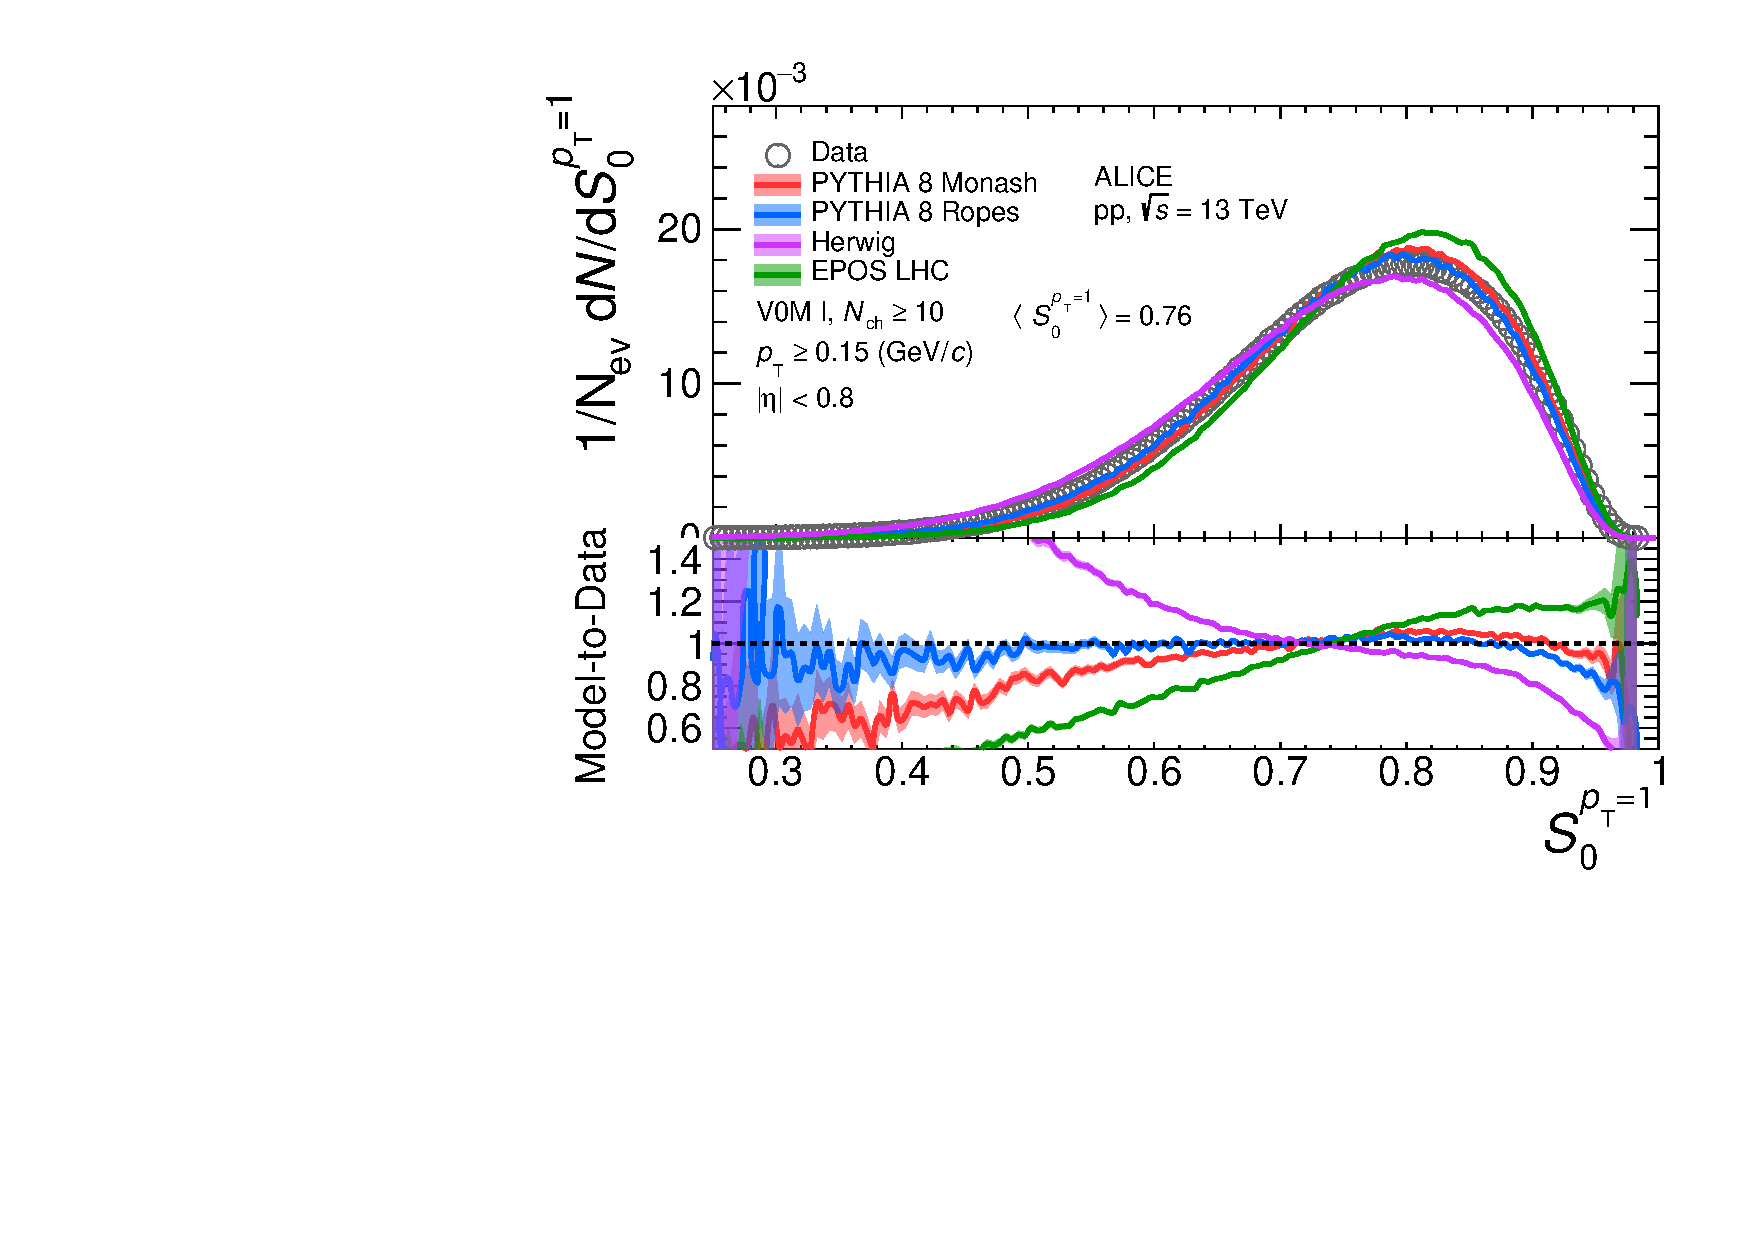
\includegraphics[width=.60\textwidth]{\imgpath/SO_Unfolded_V0M_Perc_1.pdf}}\\
\caption{The measured and fully corrected \SOPT distributions for both \textbf{(a)} \NSPD 0--1\%, \textbf{(b)} 0--10\% and \textbf{(c)} \VOM 0--1\% . The curves represent different model prediction, where the shaded area represents the statistical uncertainty of the models.}
\label{fig:sphero:sopt}
\end{figure}

\section{Transverse momentum spectra}

The corrected spectra in \VOM, and CL1 events and the dependence on spherocity for the \KOs and \LA + \AL can be seen in Fig.~\ref{fig:sphero:k0spt} and Fig.~\ref{fig:sphero:lpt}, respectively.

\begin{figure}%[!h]
\centering%
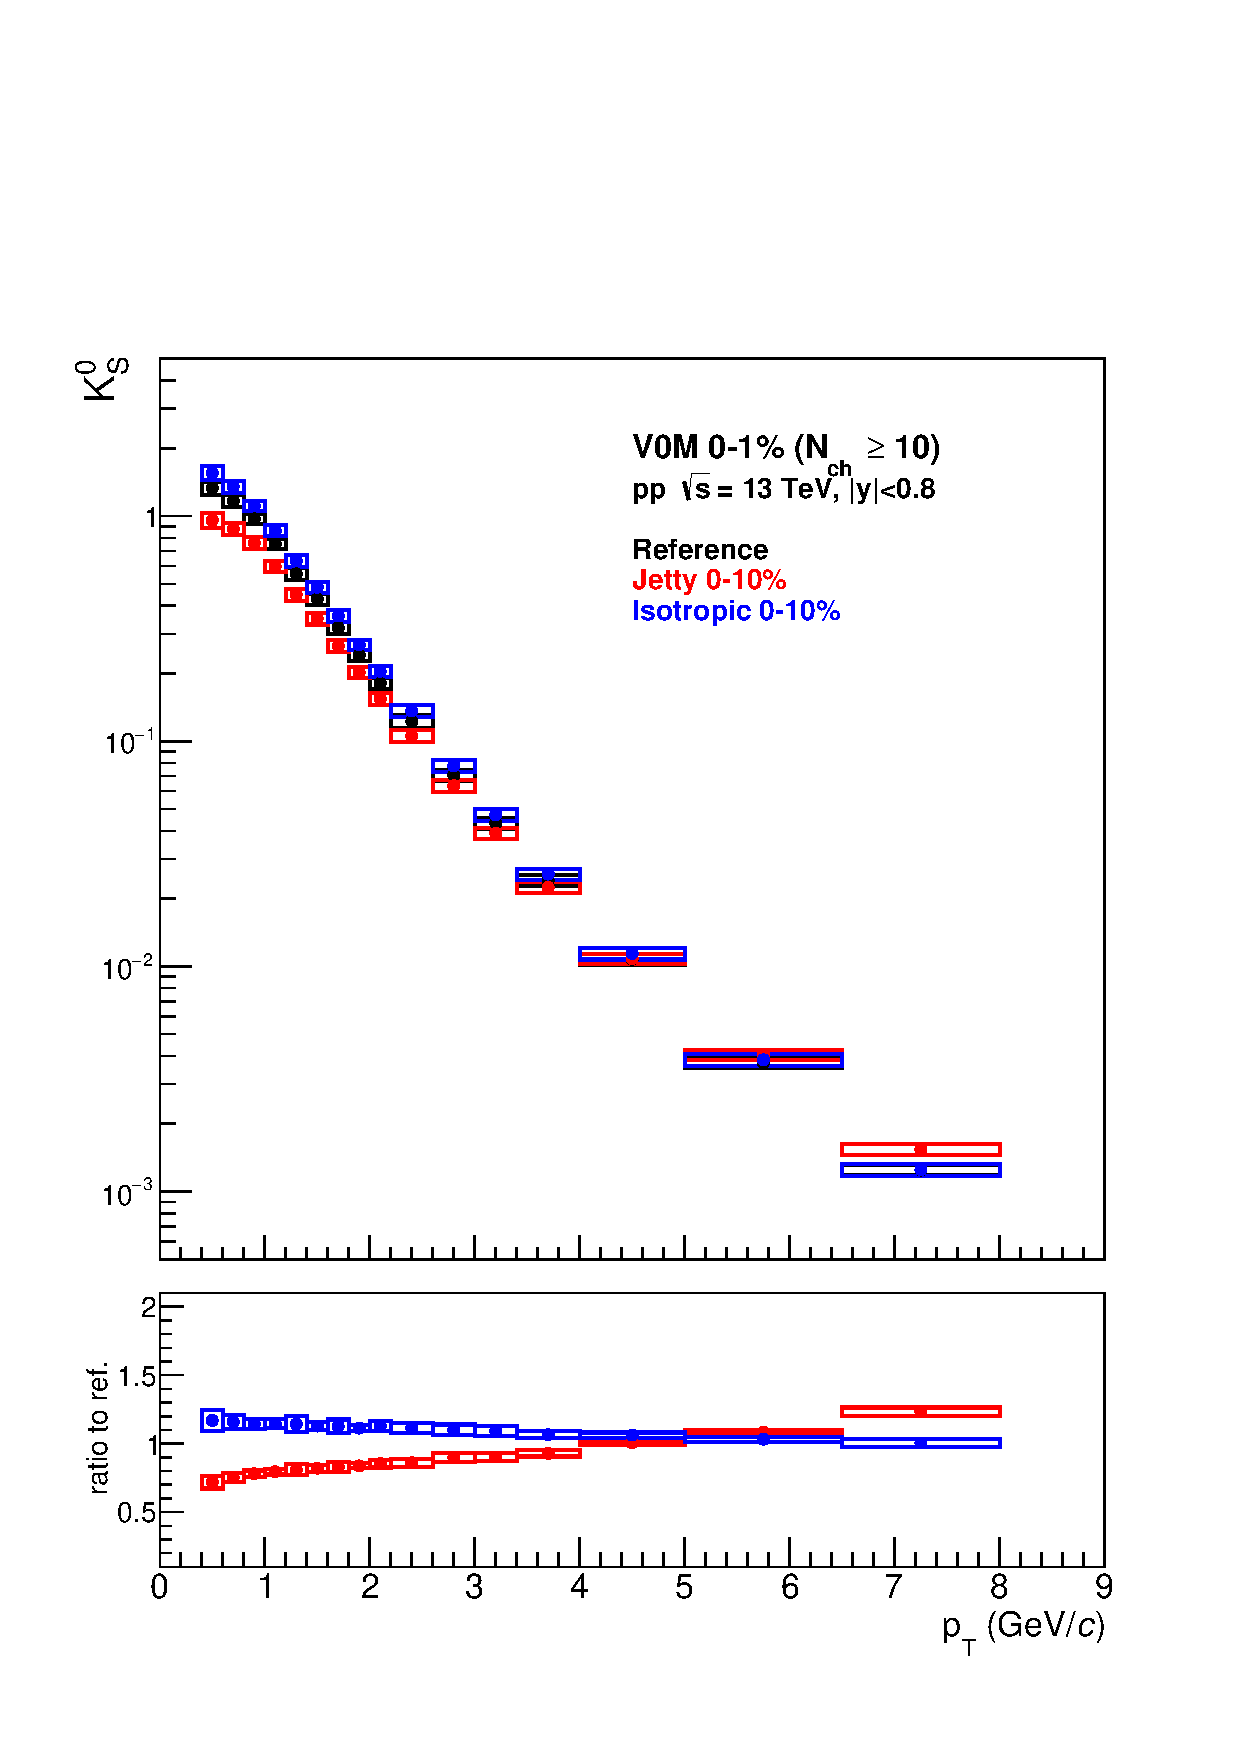
\includegraphics[height=.3\textheight]{\imgpath/sp_K0s_V0M01_spher10.pdf}
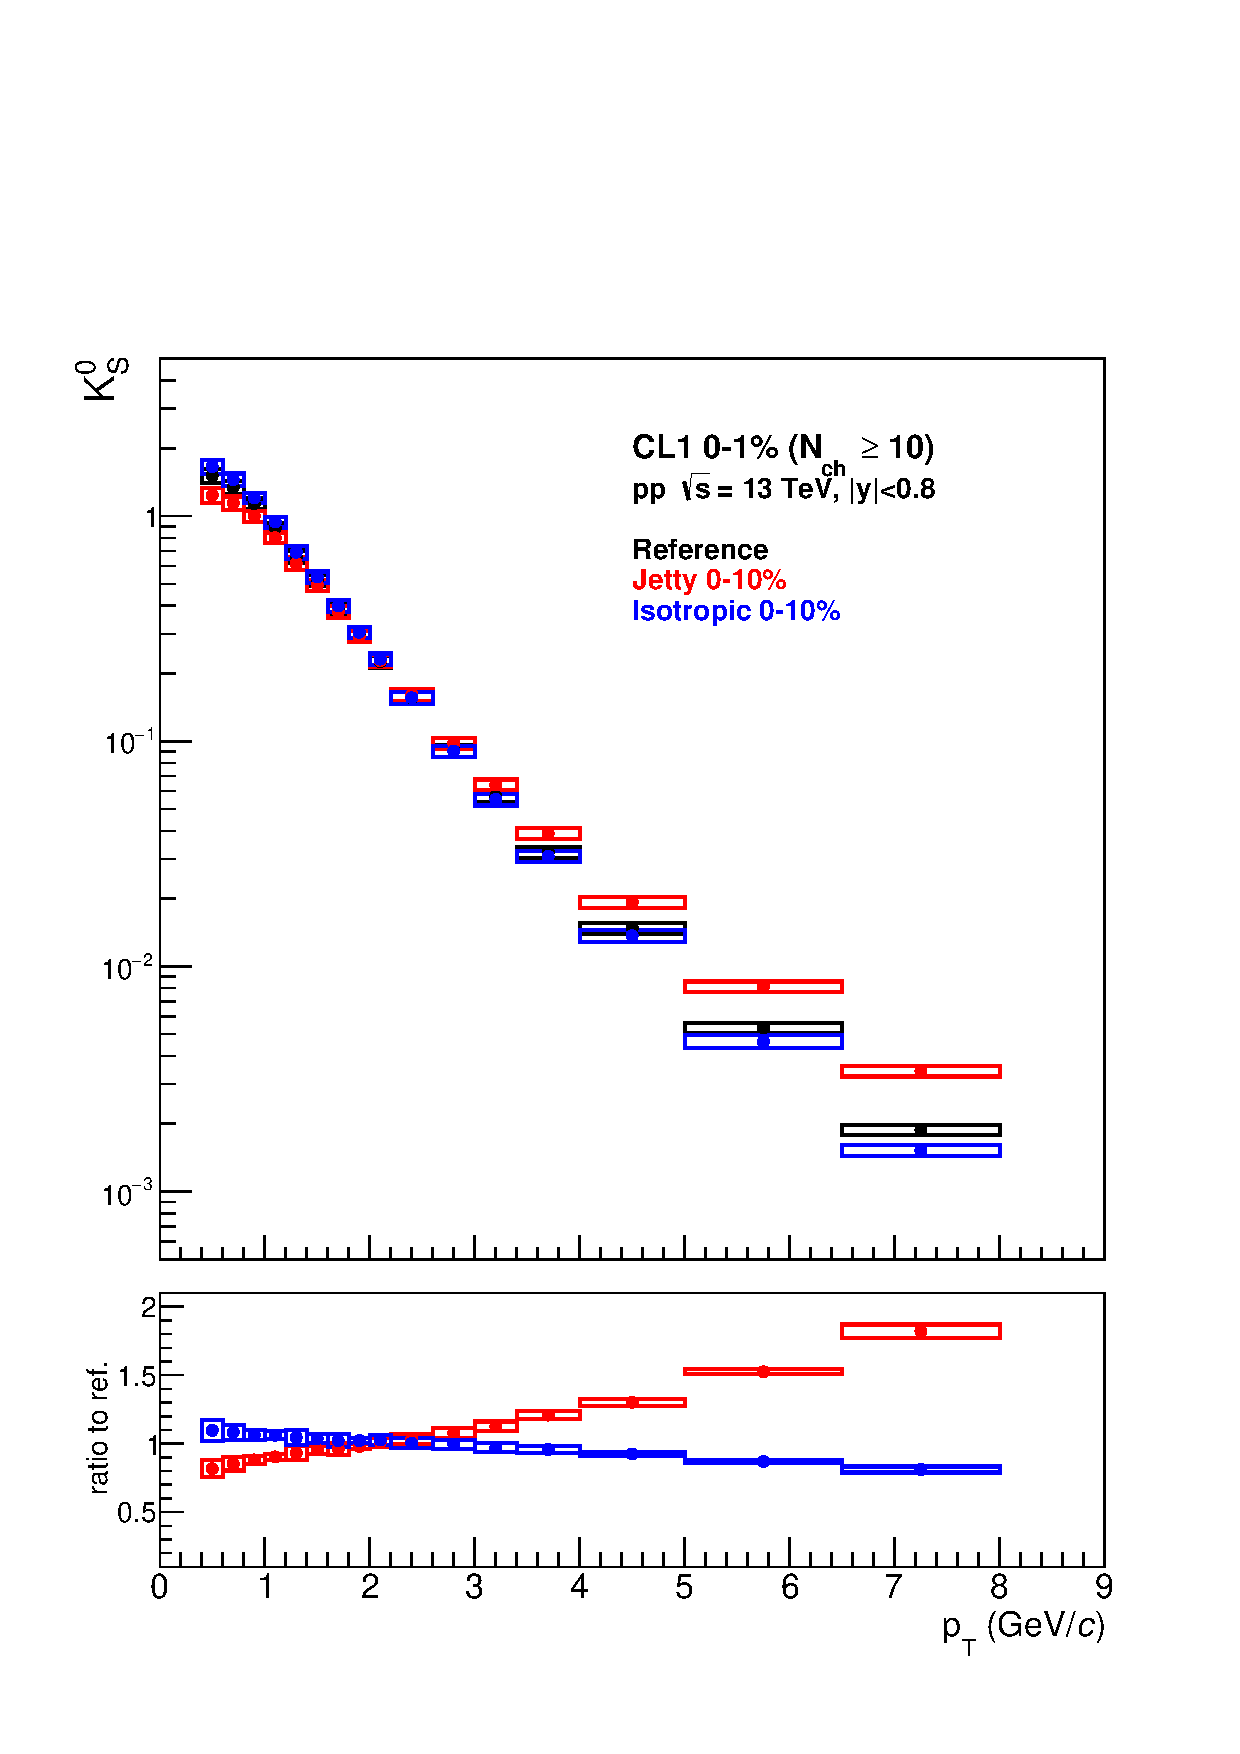
\includegraphics[height=.3\textheight]{\imgpath/sp_K0s_NCharged01_spher10.pdf}
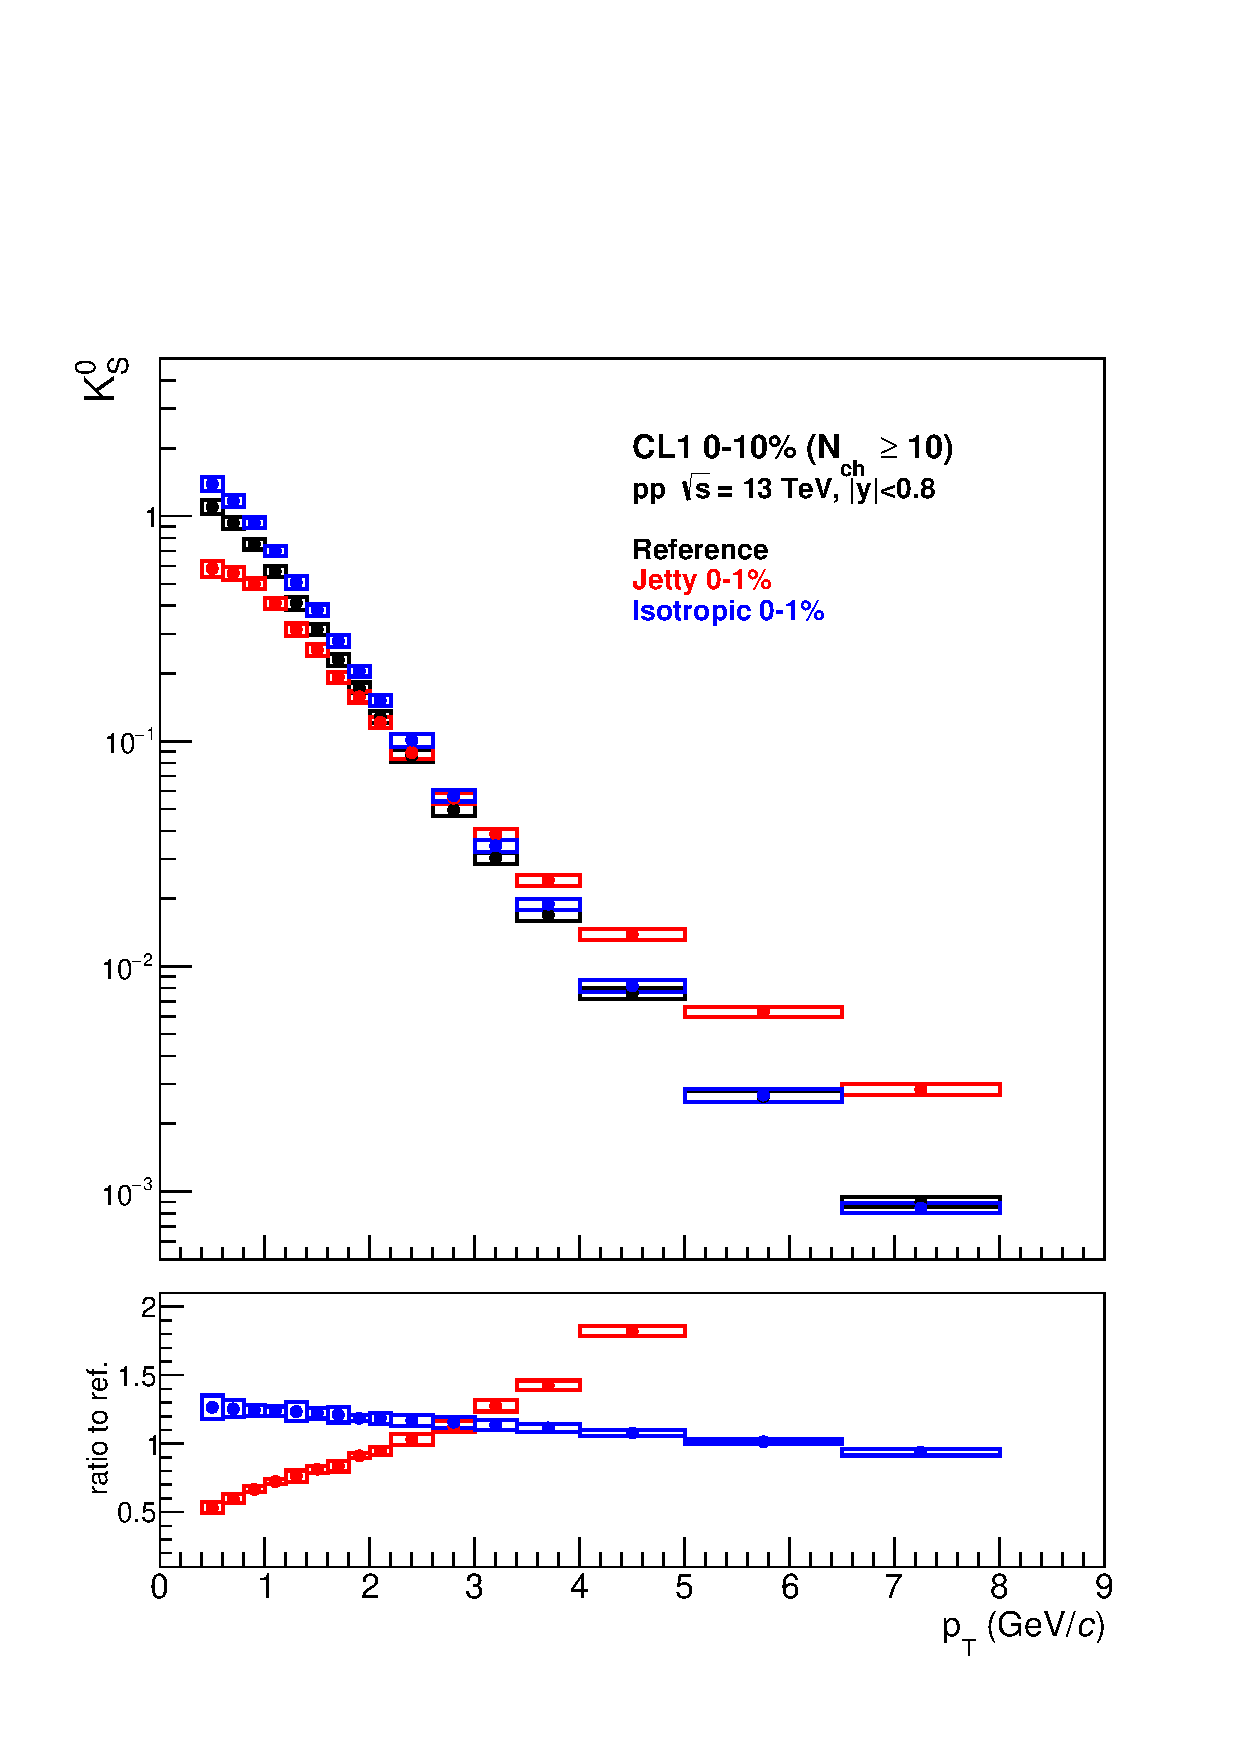
\includegraphics[height=.3\textheight]{\imgpath/sp_K0s_NCharged_spher1.pdf}
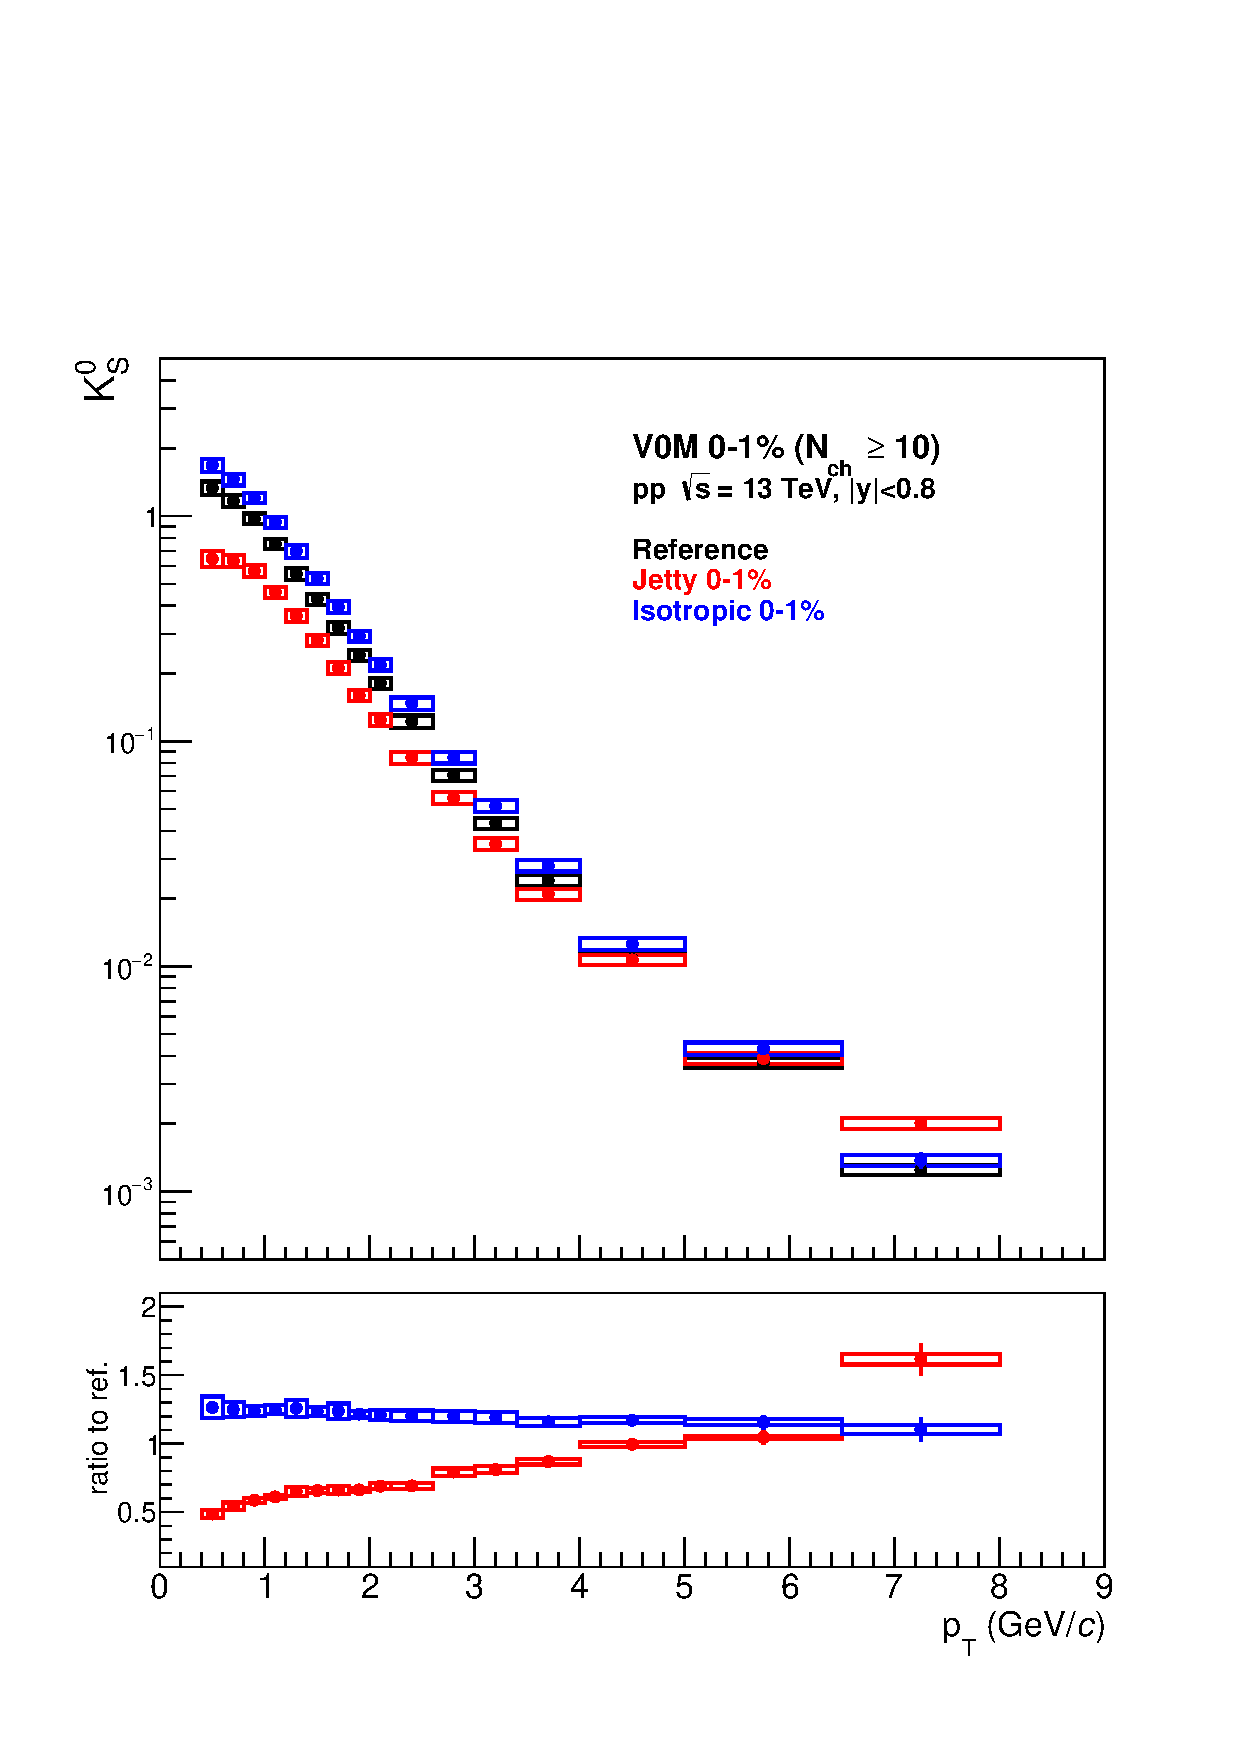
\includegraphics[height=.3\textheight]{\imgpath/sp_K0s_V0M01_spher1.pdf}
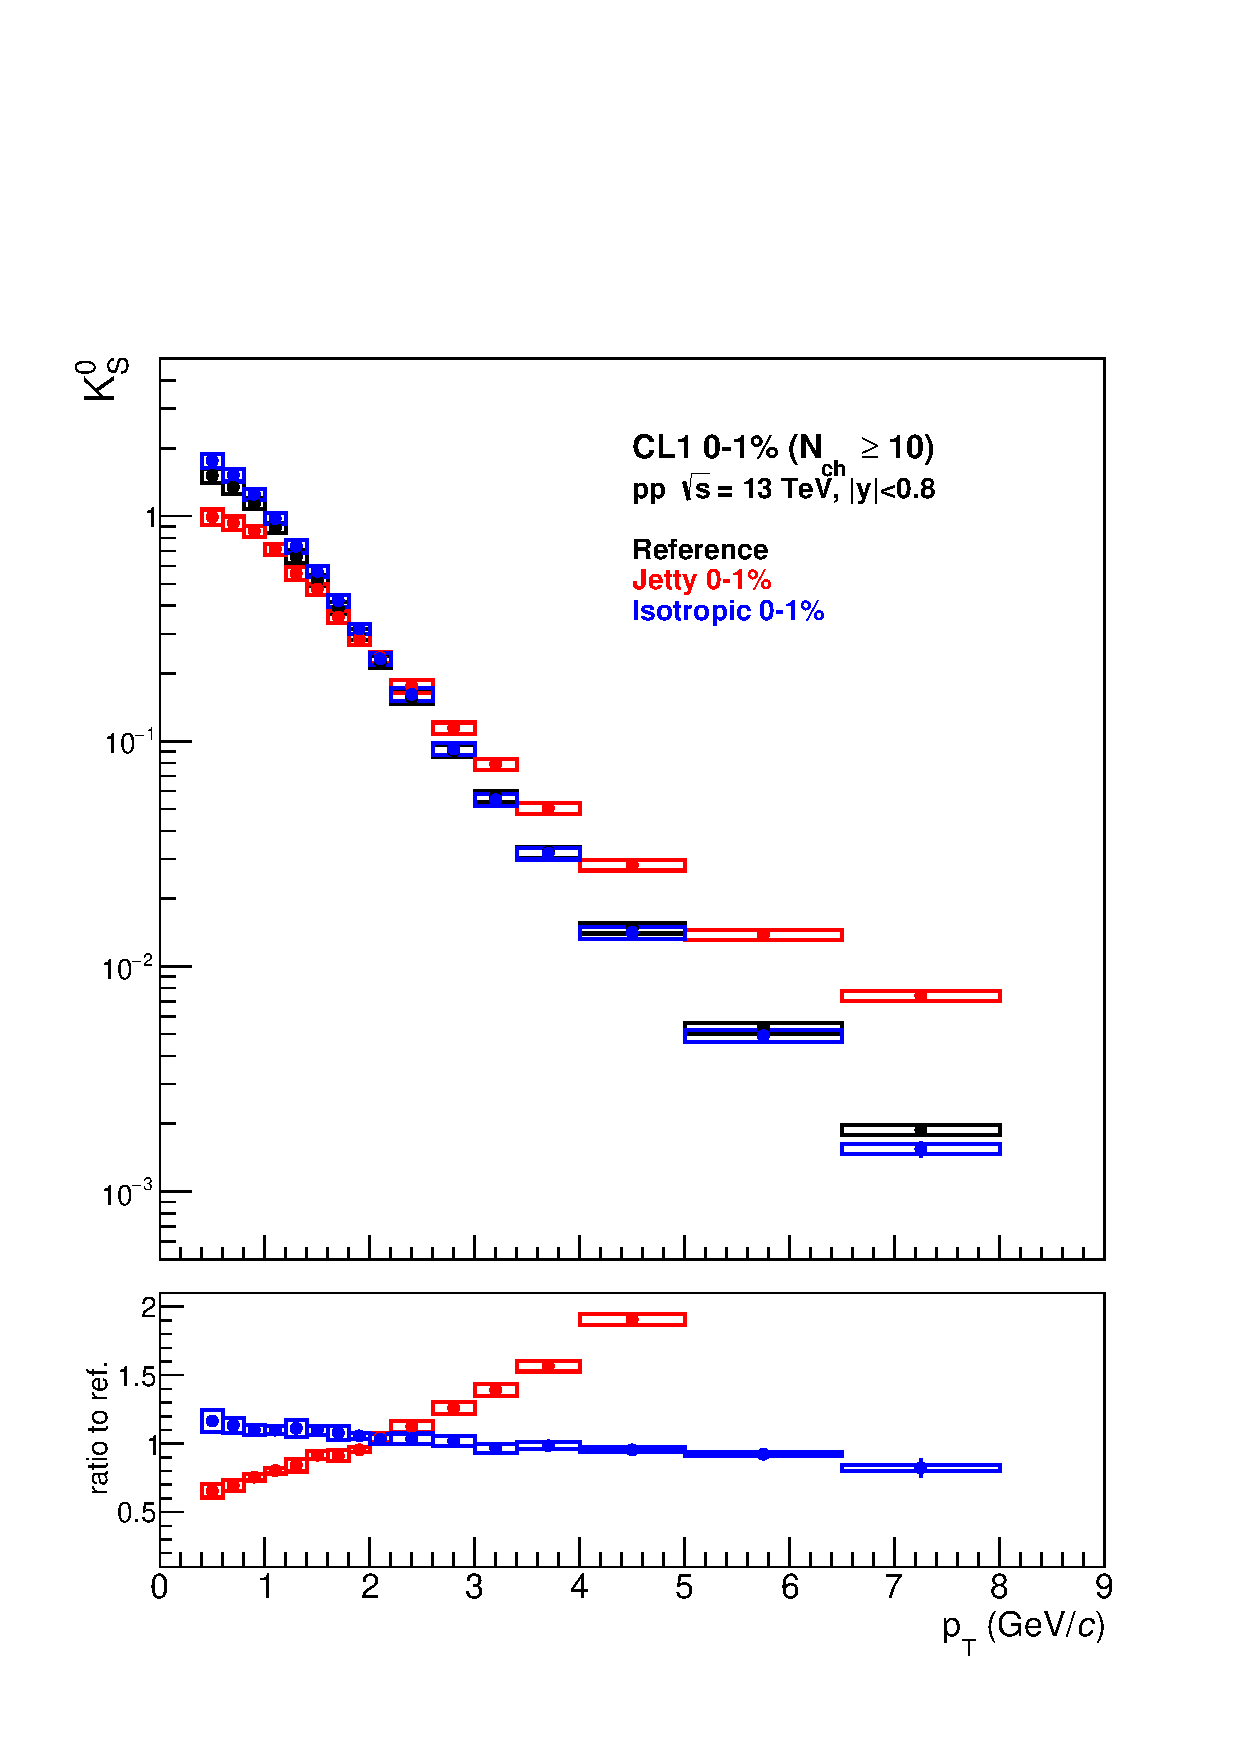
\includegraphics[height=.3\textheight]{\imgpath/sp_K0s_NCharged01_spher1.pdf}
  \caption{Corrected and normalised \pt -spectra of the \KOs particle in high-multiplicity \VOM 0-1\%(\textit{top left, bottom left}), CL1 0-1\% (\textit{top middle, bottom right}), and CL1 0-10\% (\textit{top right}) events, shown as black points. The bottom (jetty) and top (isotropic) 1\% or 10\% of spherocity events are also shown as red and blue points. The ratios of isotropic/jetty spectra to the high-multiplicity spectra are shown in the bottom panels.}
\label{fig:sphero:k0spt}
\end{figure}

\begin{figure}%[!h]
\centering%
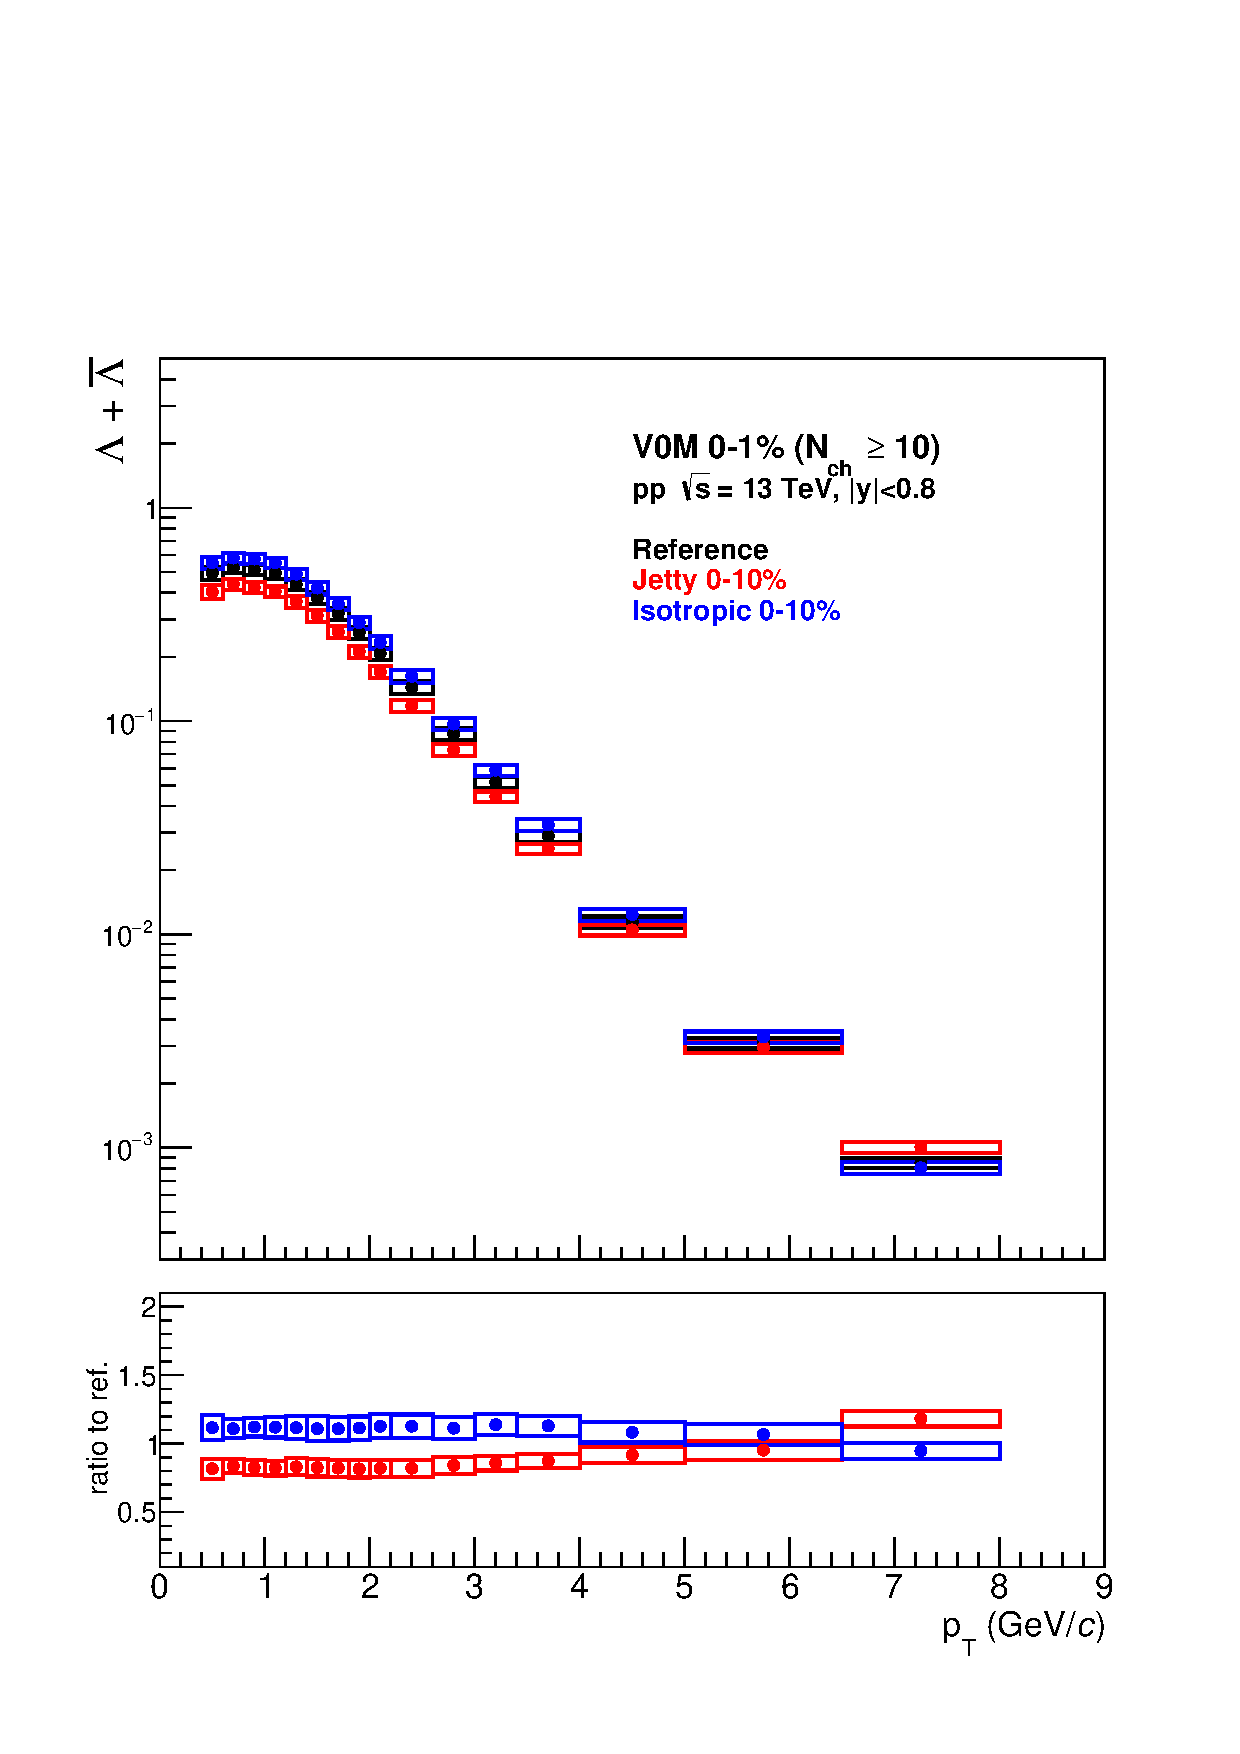
\includegraphics[height=.3\textheight]{\imgpath/sp_LLbar_V0M01_spher10.pdf}
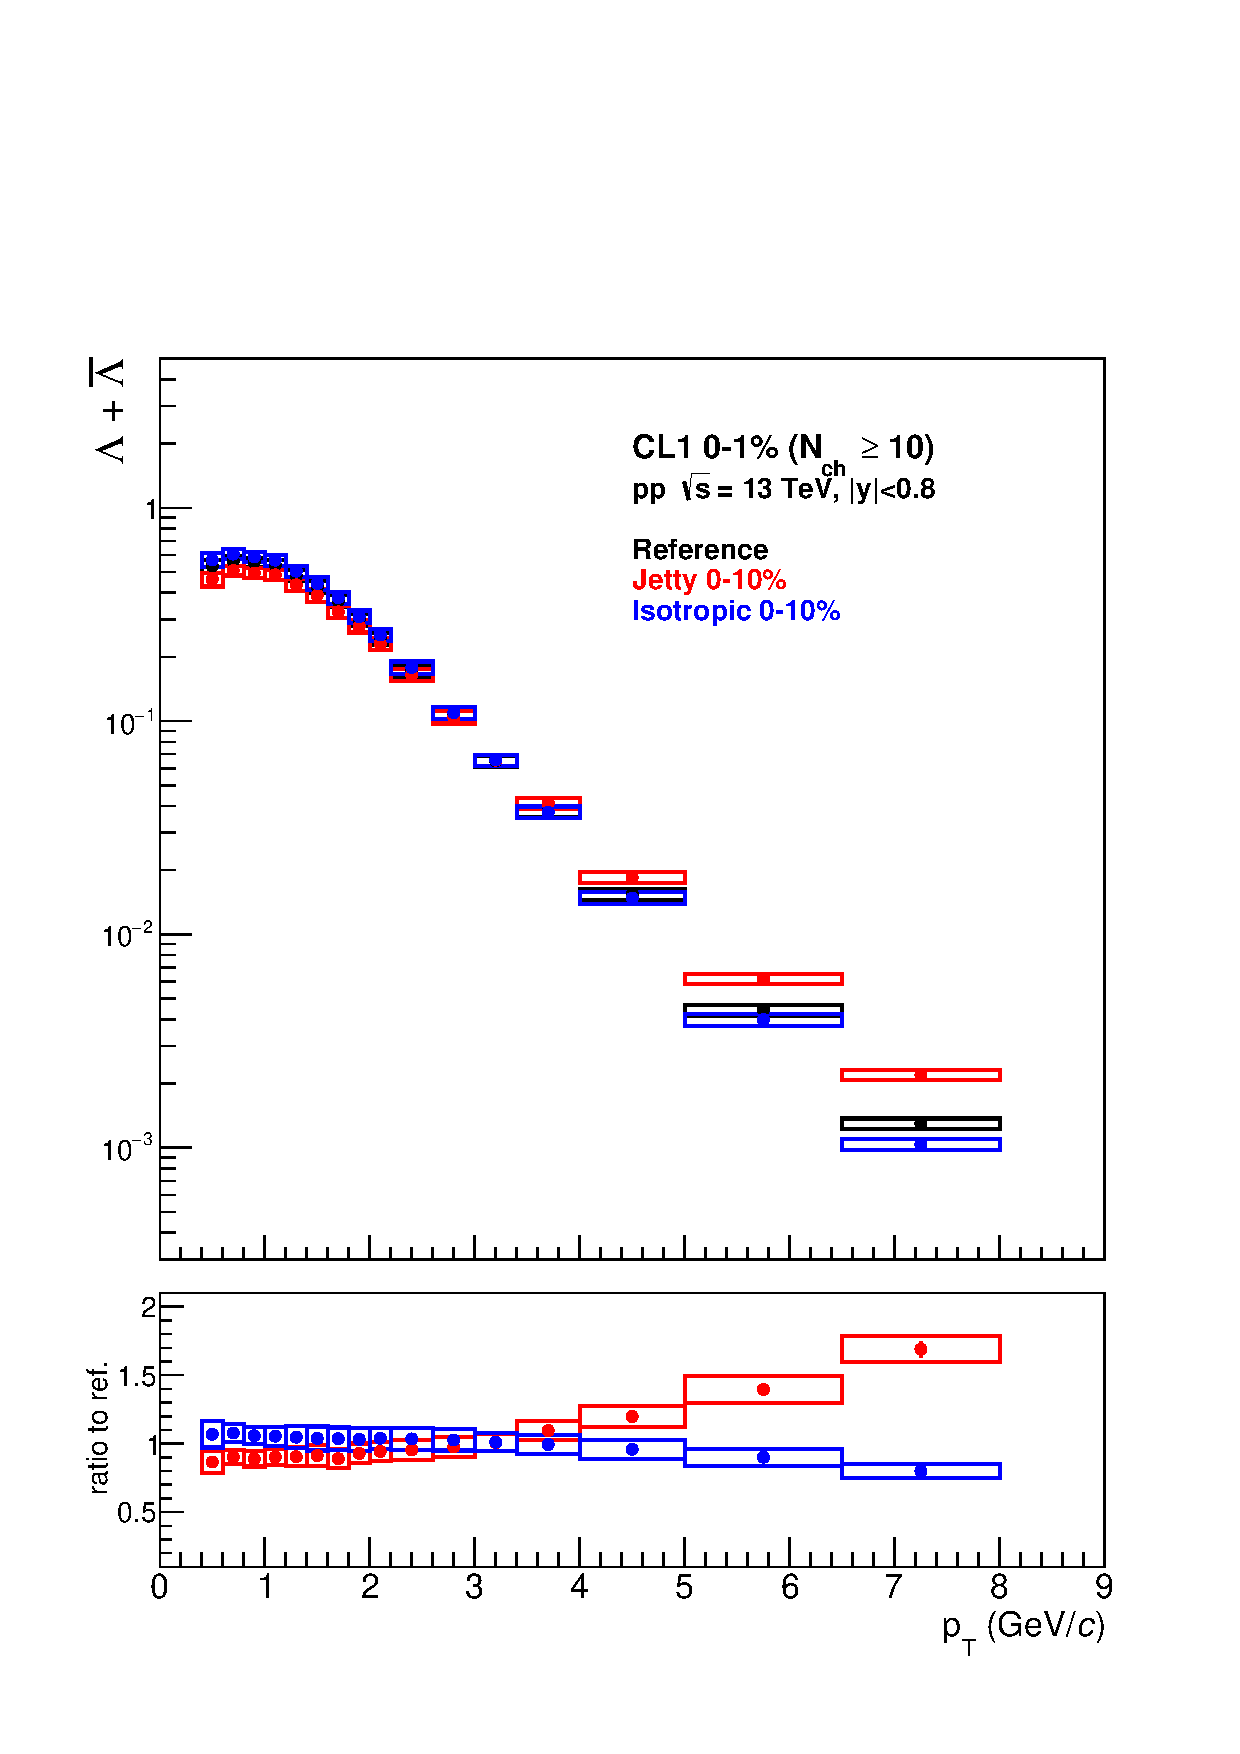
\includegraphics[height=.3\textheight]{\imgpath/sp_LLbar_NCharged01_spher10.pdf}
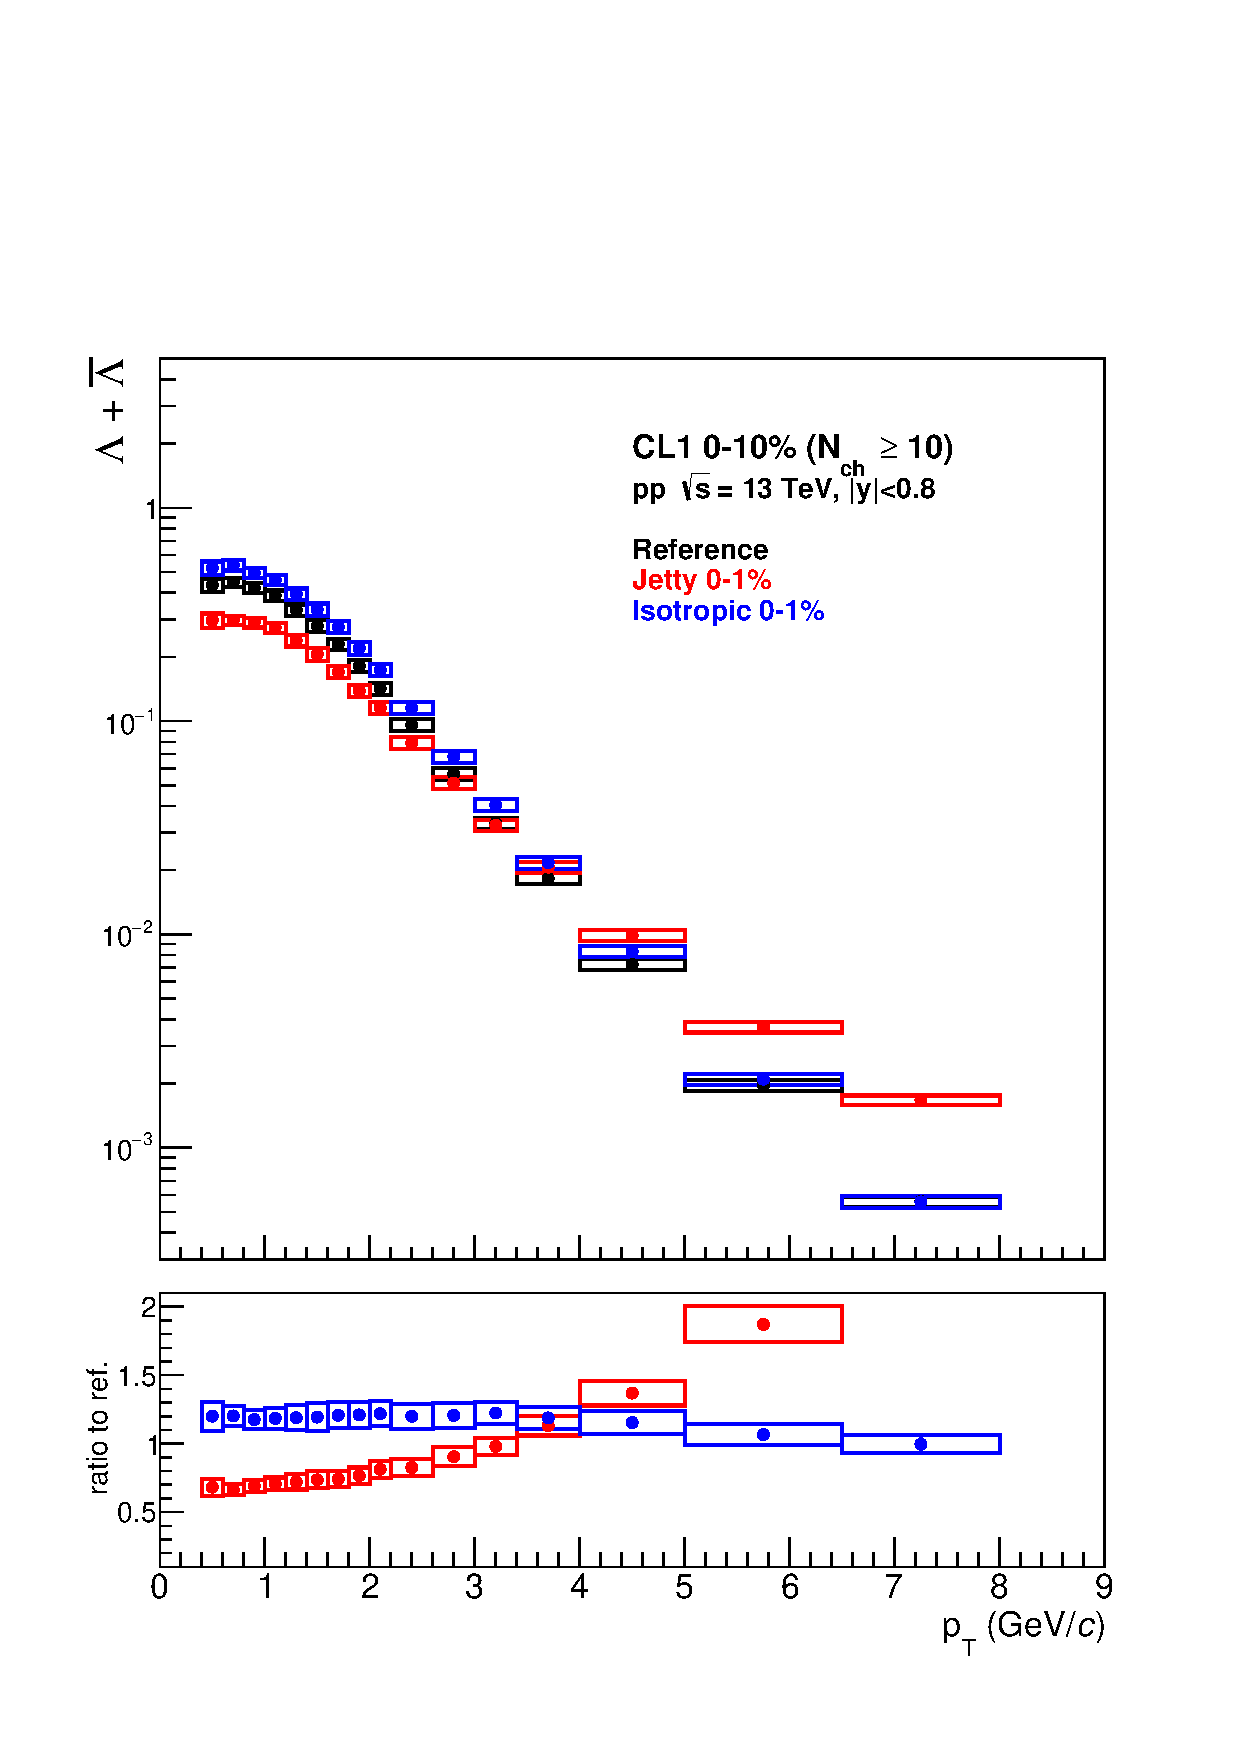
\includegraphics[height=.3\textheight]{\imgpath/sp_LLbar_NCharged_spher1.pdf}
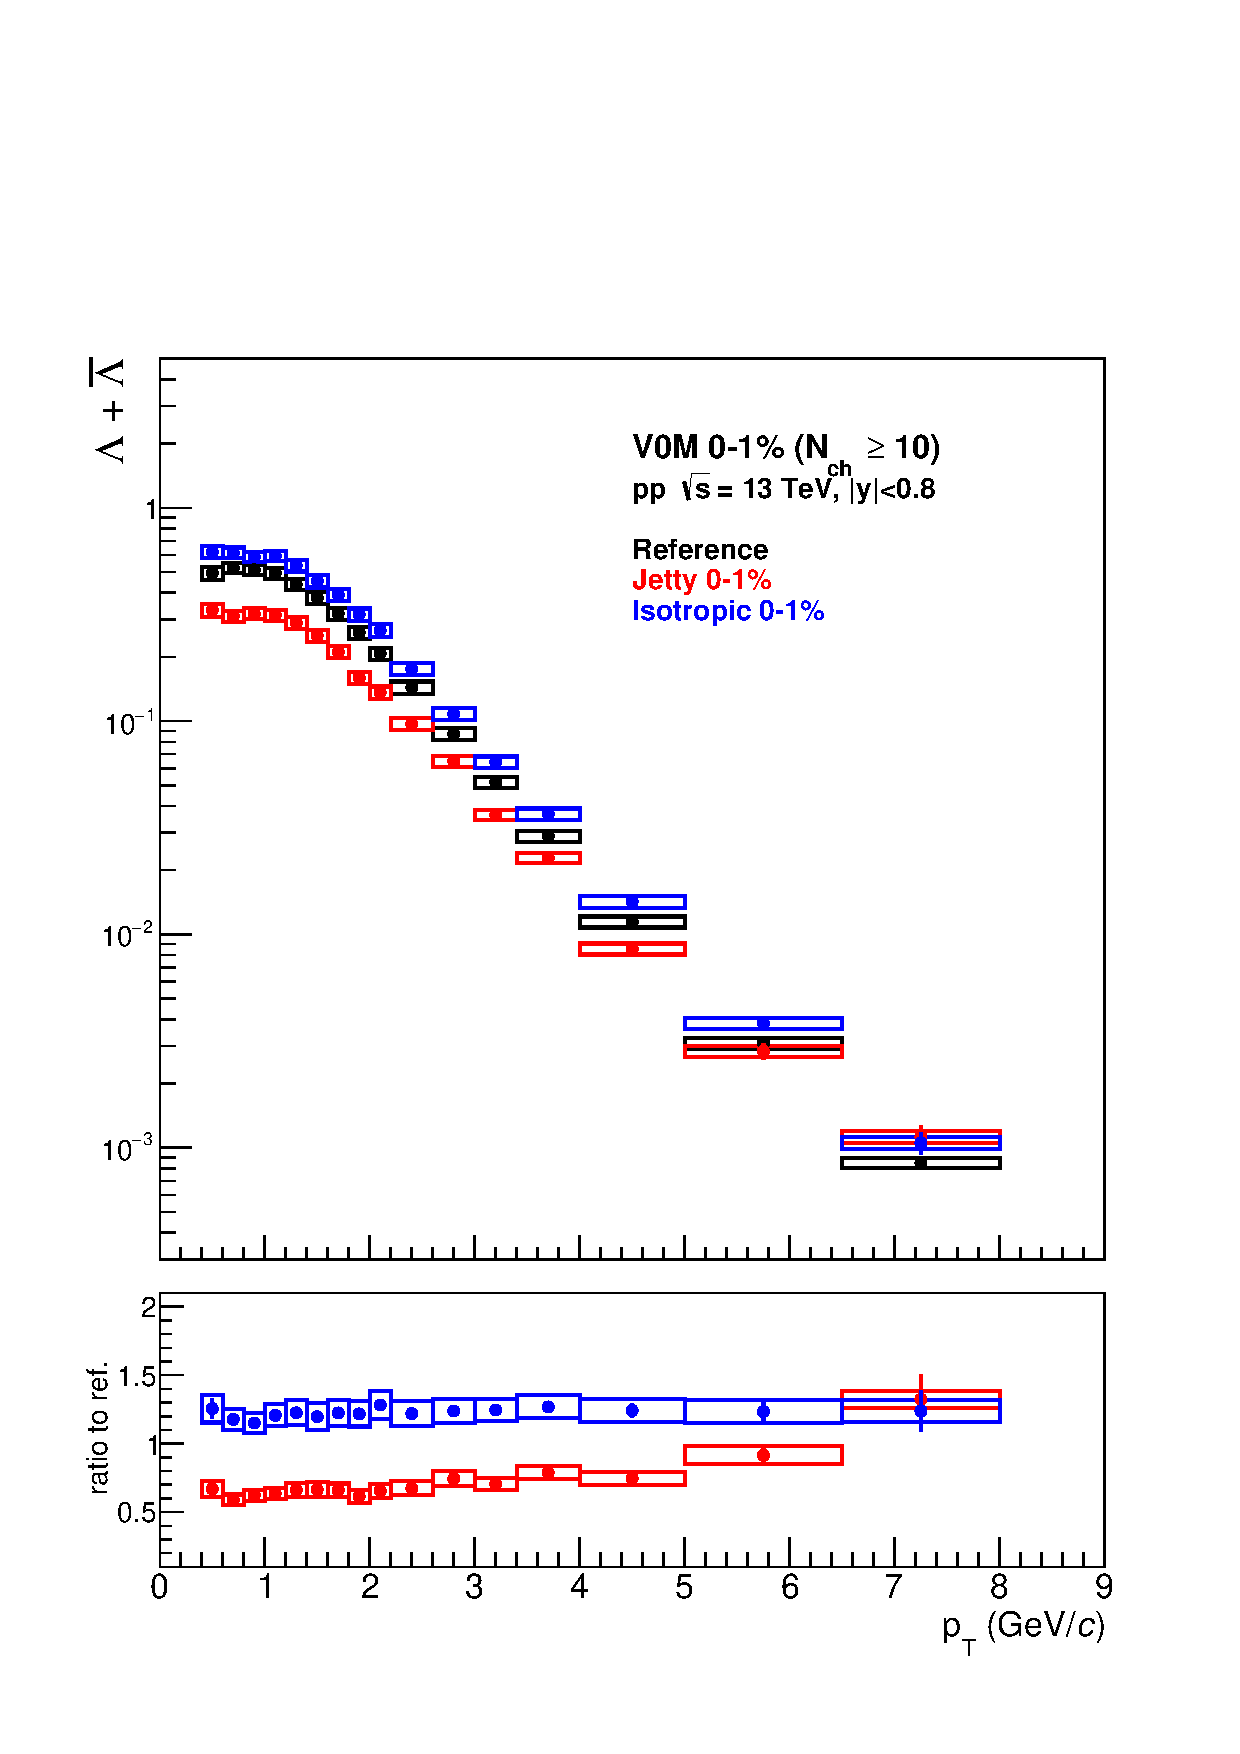
\includegraphics[height=.3\textheight]{\imgpath/sp_LLbar_V0M01_spher1.pdf}
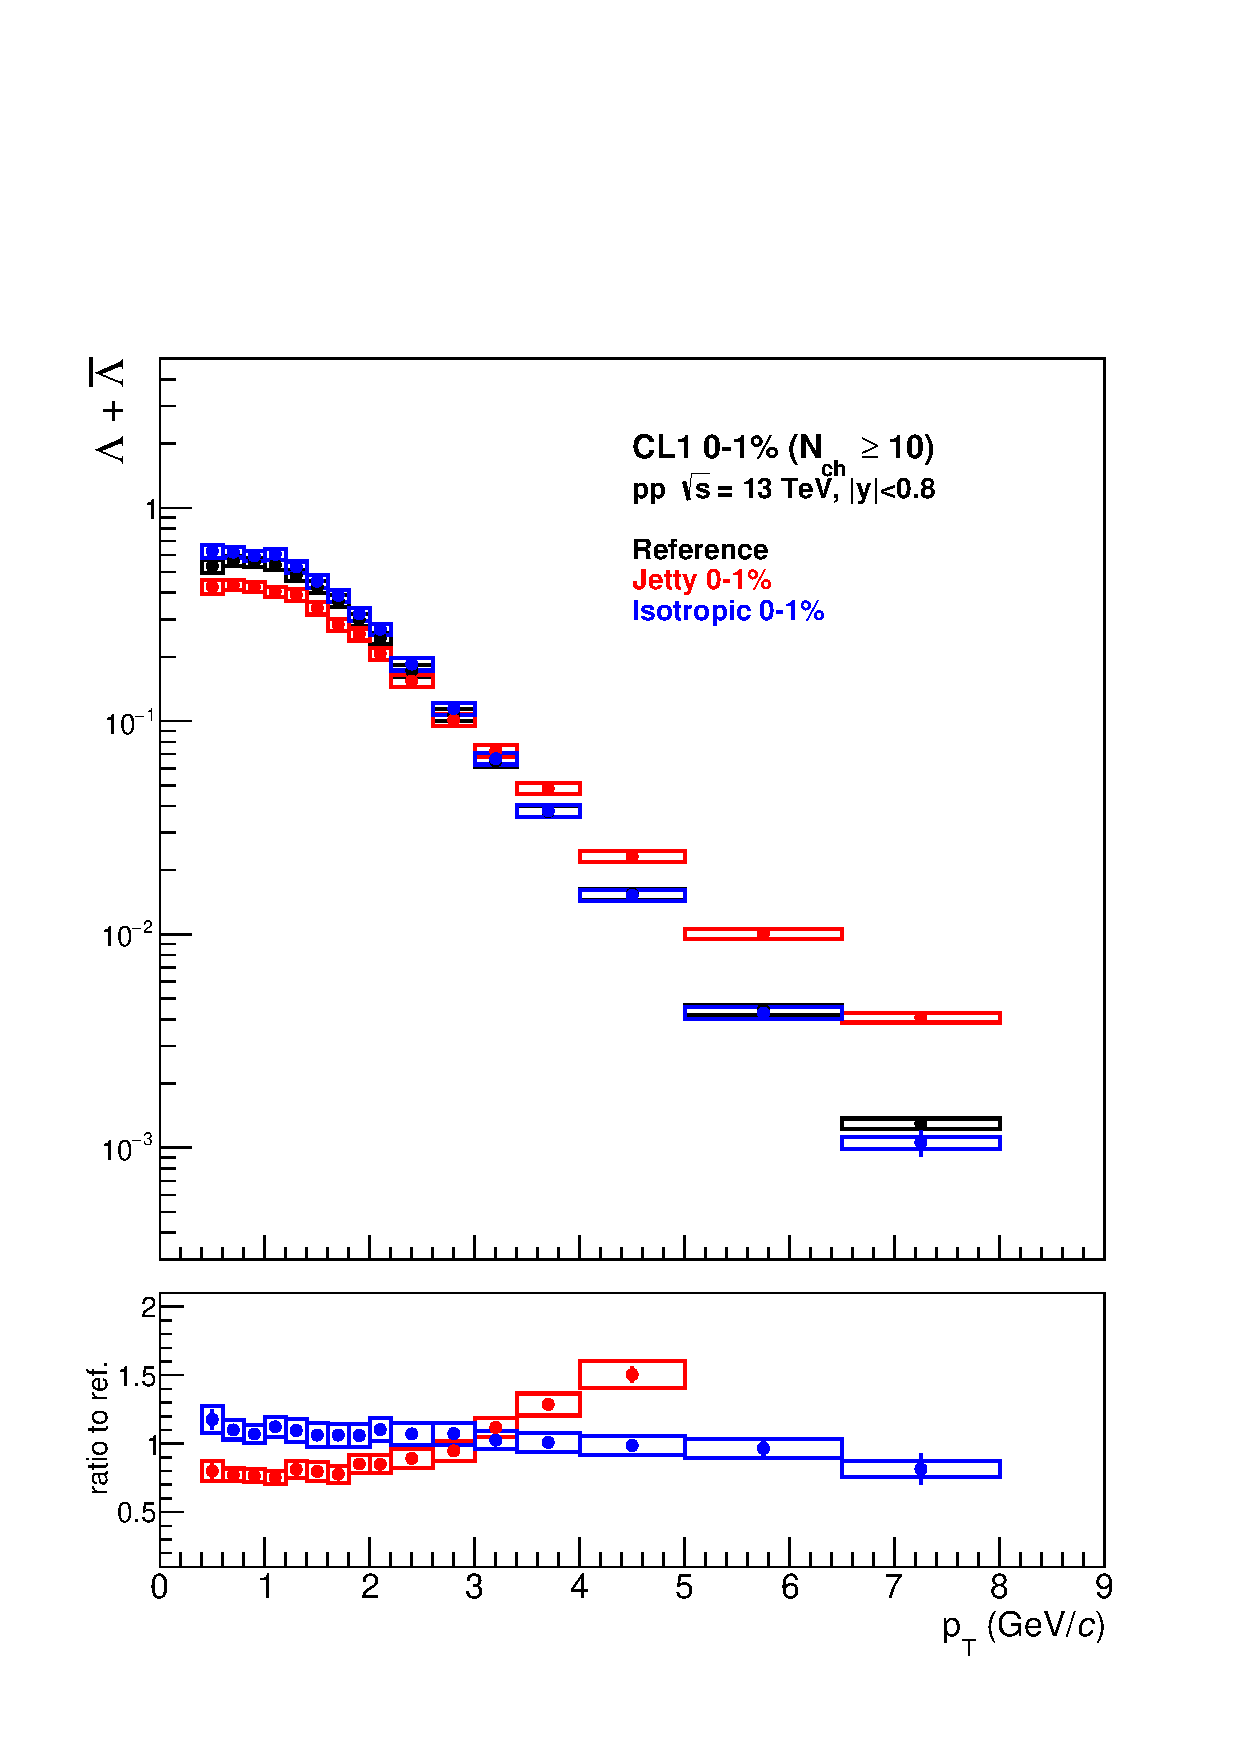
\includegraphics[height=.3\textheight]{\imgpath/sp_LLbar_NCharged01_spher1.pdf}
  \caption{Corrected and normalised \pt -spectra of the \LA + \AL particles in high-multiplicity V0M 0-1\%(\textit{top left, bottom left}), CL1 0-1\% (\textit{top middle, bottom right}), and CL1 0-10\% (\textit{top right}) events, shown as black points. The bottom (jetty) and top (isotropic) 1\% or 10\% of spherocity events are also shown as red and blue points. The ratios of isotropic/jetty spectra to the high-multiplicity spectra are shown in the bottom panels.}
\label{fig:sphero:lpt}
\end{figure}
